\documentclass{article}

\usepackage{amsmath, amsthm, amssymb, amsfonts}
\usepackage{thmtools}
\usepackage{graphicx}
\usepackage{setspace}
\usepackage{geometry}
\usepackage{float}
\usepackage{hyperref}
\usepackage[utf8]{inputenc}
\usepackage[english]{babel}
\usepackage{framed}
\usepackage[dvipsnames]{xcolor}
\usepackage{tcolorbox}
\usepackage{tikz}
\usetikzlibrary{patterns}
\colorlet{LightGray}{White!90!Periwinkle}
\colorlet{LightOrange}{Orange!15}
\colorlet{LightGreen}{Green!15}

\newcommand{\HRule}[1]{\rule{\linewidth}{#1}}

\declaretheoremstyle[name=Theorem,]{thmsty}
\declaretheorem[style=thmsty,numberwithin=section]{theorem}
\tcolorboxenvironment{theorem}{colback=LightGray}

\declaretheoremstyle[name=Proposition,]{prosty}
\declaretheorem[style=prosty,numberlike=theorem]{proposition}
\tcolorboxenvironment{proposition}{colback=LightOrange}

\declaretheoremstyle[name=Principle,]{prcpsty}
\declaretheorem[style=prcpsty,numberlike=theorem]{principle}
\tcolorboxenvironment{principle}{colback=LightGreen}

\setstretch{1.2}
\geometry{
    textheight=9in,
    textwidth=5.5in,
    top=1in,
    headheight=12pt,
    headsep=25pt,
    footskip=30pt
}

% ------------------------------------------------------------------------------

\begin{document}

% ------------------------------------------------------------------------------
% Cover Page and ToC
% ------------------------------------------------------------------------------

\title{ \normalsize \textsc{Topology and Differential Geometry}
		\\ [2.0cm]
		\HRule{1.5pt} \\
        \LARGE \textbf{\uppercase{A lecture note on Topology and Differential Geometry for Noob Wannabe Physicists}
		\HRule{2.0pt} \\ [0.6cm] \LARGE{} \vspace*{10\baselineskip}}
		}
        %\date{}
\author{\textbf{Author} \\ 
		Mushrafi Munim Sushmit \\
		Department of Physics, University of Dhaka \\
		}

\maketitle
\newpage

\tableofcontents
\newpage

\section*{Preface} % The asterisk prevents LaTeX from numbering the section
\addcontentsline{toc}{section}{Preface} 

This document draws primarily from the online lectures delivered by Professor Sunil Mukhi, which are available on YouTube. Many of the definitions, proofs, and certain sections are directly sourced from his book, Lectures on Advanced Mathematical Methods for Physicists. For more rigorous proofs go through Lecture Notes on Elementary Topology and Geometry by Itzhak Singer and John Thorpe.

\newpage 


% ------------------------------------------------------------------------------

\section{Topology}

Let's start with basic function definitions. 

\textbf{Surjective :} There is always an $ a \in A $ such that $ \forall b \in B $ there is a functional mapping from $ A :\rightarrow B $ \\ 
\textbf{Injective :} $ \forall a \in A $ and $ \forall b \in B $ there is an one to one functional mapping $ A :\rightarrow B $ \\ 
\textbf{Bijective :} When both Surjective and Injective work. that means $
\forall a \in A, \forall b \in B
$ we have $ f(a) = b $

\subsection{Topological Space}
The motivation is to capture the concept of continuity without assuming calculus. This is an 19th century development. Physicists want to capture a more general structure without using calculus such that this new thing can be used in both calculus and some other stuffs. 

We should first shed off the idea of Vector spaces or other mathematical structure. It will be helpful to consider the whole idea of Topological space as an abstract space that can accomodate any mathematical spaces. 

To start off our journey, let's try to define the limit we studied in calculus in Topology.We will try to generalize the concept of limit and continuity such that it can be used in a more generalize fashion. 

\begin{theorem}
  An open set is defined as $ x \in X \rightarrow x \in (a,b) \subset X $
\end{theorem}

What it means is that if we take any elements from $ X $ it will always be smaller than a fixed boundary or greater than a fixed boundary. Another way to look at it is the limits. If we consider an open set in the interval $ x \in (a,b) $ or maybe an infinite set $ x \in (a,\infty) $ then we can always choose a point $ x  $ such that $ | x-a|< \epsilon $
and $ |b-x| < \epsilon $ is always satisfied. \textbf{All points in that set should have the value such that they can be enclosed by an open interval (a,b) }

\begin{theorem}
    A closed set is the compliment of open set.     
\end{theorem}

To prove that the $ x \in [a,b] \subseteq A $ is an element of closed set we take the compliment of $ A $ and we will get $ x \in (\infty, a) \cup  x \in (b,\infty) $. Clearly the latter is an open set so by definition, $ A $, as it is the compliment of an open set, must therefore be a closed set.   

Examples of open set include empty set, Real numbers set, any number line extended to infinity.

Examples of closed set are single points, closed intervals. Even the real numbers and empty sets are also closed sets. They are kind of both open and closed due to the definition. 

A set can be open, closed, both or neither. So it's better not to hung up on this notion. Just treat it as it is. Another thing to keep in mind is that we are dealing with sets not just fixed intervals. 

Now if we combine all of this the formal definition of Topology is thus 

\begin{theorem}
    Let S be an non-empty set and U be a collection of subset of X satisfying the following three conditions 
    \begin{enumerate}
        \item $ \phi \in U, S \in U $ 
        \item For any two subsets $ S_1 \in U $ \& $ S_2 \in U $, then $ S_1 \cap S_2 \subset U $ 
        \item For any two subsets For any two subsets $ S_1 \in U $ \& $ S_2 \in U $, then $ S_1 \cup S_2 \subset U $ 
    \end{enumerate} 
    Then $ (S,U) $ is called the Topological space and the collection $ U $ is called the Topology on $ S $ 
\end{theorem}

We are free to choose the Topology $ U $, we can choose whatever set we want as long as the above conditions are satisfied. 

\begin{proposition}
    Let $ X = {a,b,c} $ and $ T = \{ \phi, X, \{a\}, \{b\}, \{a,b\} \} $ then T is a Topology. but if we had $ T = \{ \phi, X, \{a\}, \{b\}, \{a,b\} , \{c\} \} $, Then this is not a topology. 
    Cause the union of $ \{b\} \cup \{c\} = \{b,c\} \notin T $ 
\end{proposition}

Some definitions 

\begin{itemize}
    \item \textbf{Indiscreet Topology :} When the Topology of Topological space $(S,U)$ involves only the empty set $\phi$ and $S$ 
    \item \textbf{Discreet Topology :} When the topology involves all the subsets possible 
        (power set) 
\end{itemize}

\subsection{Metric Space}
A \textbf{metric space} is a set $M$ together with a function $d: M \times M \to \mathbb{R}^{+}$, called a $\emph{metric}$ or $\emph{distance function}$, such that for all $x, y, z \in M$, the following conditions are satisfied:
\begin{enumerate}
    \item \textbf{Non-negativity:} $d(x, y) \geq 0$.
    \item \textbf{Identity of indiscernibles:} $d(x, y) = 0$ if and only if $x = y$.
    \item \textbf{Symmetry:} $d(x, y) = d(y, x)$.
    \item \textbf{Triangle inequality:} $d(x, z) \leq d(x, y) + d(y, z)$.
\end{enumerate}

It is basically a measuring device. We are all too much engrossed with the cartesian distance formula, which is not necessarily the only formula or the correct formula to measure distance in a higher plane or in a different coordinate system. The above abstract definition allows for a more general set of formulas and is useful. Minkowski space is not a metric space as it violates the above conditions. 

An example of metric space is, on $\mathbb{R}$, we may choose the usual metric $d(x, y) = |x - y|$.     


Now why did we mention this space. Metric space can be used to define a topology. 

\section*{Metric Topology}

Let's start with a \textbf{metric space}. A metric space consists of a set $X$ along with a function $d: X \times X \to \mathbb{R}$, called a \emph{metric}, which measures the distance between any two points in $X$. The \textbf{metric topology} is a way of defining which subsets of $X$ can be called "open". An open set in this context is a set where, for any point within it, you can find a small "neighborhood" around that point which is entirely contained within the set. 

Formally, 

\begin{theorem} 
Let $(X, d)$ be a metric space where $X$ is a set and $d: X \times X \to \mathbb{R}$ is a metric. The \textbf{metric topology} on $X$ is the topology $\mathcal{T}$ generated by the open sets defined using the metric $d$. A subset $U \subseteq X$ is said to be \emph{open} in the metric topology if, for every point $x \in U$, there exists an $\epsilon > 0$ such that the open ball $B_d(x, \epsilon) \subset U$. Here, the open disc $B_d(x, \epsilon)$ is defined as
\[
B_d(x, \epsilon) = \{ y \in X \mid d(x, y) < \epsilon \}.
\]

\end{theorem}

To think of an open disc consider the points enclosed by a circle, but now the boundaries are not inlcuded, means they have an open interval. But it is abstract and defined by the metric. 

The metric topology defines a structure on $X$ that allows us to talk about concepts like continuity, convergence, and compactness in a rigorous way. It turns our set $X$ into a \emph{topological space}, which means it satisfies three key properties:
\begin{enumerate}
    \item The set $X$ itself and the empty set $\emptyset$ are considered open.
    \item Any union of open sets is also open.
    \item Any finite intersection of open sets is also open.
\end{enumerate} 

Examples are given below:
\begin{enumerate}
    \item In the real numbers $\mathbb{R}$, we can define the distance between any two points $x$ and $y$ as $d(x, y) = |x - y|$. The open sets in this metric topology are unions of open intervals, like $(a, b)$, where $a < b$.

    \item In the plane $\mathbb{R}^2$, we define the distance between points $(x_1, y_1)$ and $(x_2, y_2)$ as
    \[
    d((x_1, y_1), (x_2, y_2)) = \sqrt{(x_1 - x_2)^2 + (y_1 - y_2)^2}.
    \]
    The open sets in this metric topology are unions of open disks (circles without the boundary).
\end{enumerate}

It's convenient to use a matric space to define a topology but not the necessity.

\subsection{Topology Basis} 

To understand the concept of a topology, we need to introduce the idea of a \textbf{basis}. A basis helps us define a topology in a more manageable way by specifying a set of "building blocks" for the open sets.

The open intervals on \(\mathbb{R}\) have the following properties:
\begin{itemize}
    \item[(i)] The union of all open intervals is the whole set \(\mathbb{R}\):
    \[
    \bigcup (a_i, b_i) = \mathbb{R}
    \]
    \item[(ii)] The intersection of two open intervals can be expressed as the union of other open intervals. For example, if \(a_1 < a_2 < b_1 < b_2\), then
    \[
    (a_1, b_1) \cap (a_2, b_2) = \bigcup (a_2, b_1)
    \]
    \item[(iii)] \(\emptyset\) is an open interval: \((a, a) = \emptyset\).
\end{itemize}
These properties can be abstracted to define a basis for an arbitrary topological space. 

\begin{theorem}
  In an arbitrary topological space (S, U), any collection of open sets
(a subset of the full collection U) satisfying the above three conditions is called
a basis for the topology.

\end{theorem}

The topology is not the set of all open disks. Only the collection that obeys the topology properties. The union of open disks also need not be an open disk. A point to note if we keep on taking infinite intersections, it is possible to get a non open set or a closed set or a specific value perhaps. Thus in the definition of Topology, the union can be of any infinite sets but the intersection must be of finite order. Thus the intersection of two open disks may or may not be an open disk. 

one example would be $  ( \frac{1}{-n}, \frac{1}{n} ) $, If we keep on taking infinite intersections while increasing n, the final outcome can only be $ \{ 0 \} $ which is an closed set. 

\subsection{Closure}
To define a limit or a boundary for an open set, we can consider small points, s outside the open discs A, for which no matter how small disks we make around s, it intersects with A. 

\begin{theorem}
    Let $(S, \mathcal{U})$ be a topological space. Let $A \subseteq S$. A point $s \in S$ is called a limit point of $A$ if, whenever $s$ is contained in an open set $u \in \mathcal{U}$, we have
\[
(u \setminus \{s\}) \cap A \neq \emptyset.
\]
\end{theorem}

According to the description above, any points inside A can be a limit point of A, But for outside A, the only option that can be the limit point is the boundaries. These points are called the closure of A. 

\begin{theorem}
The closure of a set $A \subseteq S$ is:
\[
\bar{A} = A \cup \{ \text{limit points of } A \}.
\]
\end{theorem}

Which in turn means that the closure of a set is a closed set. 

\subsection{Connected Space}

To define connected space, we first define disconnected space. And logically if we cant prove two sets are disconnected, then they must be connected.  

\begin{theorem}
 A topological space $(S, \mathcal{U})$ is connected if it cannot be expressed as the union of two disjoint open sets in its topology. If, on the other hand, we can express it as the union of disjoint open sets — that is, if there exist open sets $U_1, U_2 \in \mathcal{U}$ such that $U_1 \cap U_2 = \emptyset$ and $U_1 \cup U_2 = S$ — then the space is said to be disconnected.
\end{theorem}

So we cannot write a connected topological space with open sets. It is intuitive in the sense that for open sets, we never define or count the boundary region. So if two sets are not connected, how could they be considered continuous. 

Connectedness depends on the topology. Cause we are looking at open and closed sets to come up with whether they are connected or not. 

\begin{theorem}
    The discrete topology on a set \( S \) is defined as the topology where every subset of \( S \) is open. Formally, the discrete topology \( \mathcal{U}_{\text{discrete}} \) on \( S \) is given by \( \mathcal{U}_{\text{discrete}} = \{ U \subseteq S \mid U \text{ is any subset of } S \} \).

In the discrete topology: 
\begin{itemize}
    \item  Every singleton set \( \{s\} \subseteq S \) is open.
    \item Every subset of \( S \), including \( S \) itself and the empty set \( \emptyset \), is open.
   \item The closure of any subset \( A \subseteq S \) is \( \bar{A} = A \), since every point of \( A \) is a limit point of \( A \) itself in this topology.
\end{itemize}
\end{theorem}

The discrete topology is the finest (or most refined) topology possible on \( S \), meaning it is the topology with the greatest number of open sets. It provides the maximum degree of flexibility and granularity in defining open sets. 

Now we move onto the study of closed, bounded sets. Before we begin let us define the cover. 

\subsection{Cover and Compactness}

\begin{theorem}
    \textbf{Definition:} A cover of a set \( X \) is a family of sets \( \{ F_\alpha \} = \mathcal{F} \) such that their union contains \( X \). Formally,
\[
X \subset \bigcup_{\alpha} F_\alpha.
\]

If \((S, \mathcal{U})\) is a topological space and \( X \subset S \), then a cover \( \{ F_\alpha \} \) is said to be an open cover if \( F_\alpha \in \mathcal{U} \) for all \( \alpha \), namely, if all \( F_\alpha \) are open sets.

\textbf{The Heine-Borel Theorem:} In the context of \(\mathbb{R}^n\), the Heine-Borel theorem states that a subset \( X \subset \mathbb{R}^n \) is compact if and only if it is closed and bounded. This means that if \( X \subset \mathbb{R}^n \) is compact, then every open cover of \( X \) has a finite subcover. Formally, if \( \{ F_\alpha \} \) is an open cover of \( X \), then there exists a finite subcover \( \{ F_{\alpha_1}, F_{\alpha_2}, \ldots, F_{\alpha_k} \} \) such that
\[
X \subset F_{\alpha_1} \cup F_{\alpha_2} \cup \cdots \cup F_{\alpha_k}.
\]
\end{theorem}

The concept of a cover provides a way to describe how a set \( X \) can be "covered" or "contained" by a collection of other sets. An open cover is a special type of cover where all the covering sets are open in the given topology.

For compact sets or in other words bounded and closed intervals, we only need some covers that will enclose the boundary. We can always take subsets that will start from the left boundary to the right boundary and union them, thus it will always cover it. even if we only consider the inside parts of the compact set. Due to the definition of closed intervals, the boundaries must be included, as a result all points are covered by the chosen subsets of the cover even if the cover is equal or greater than the main set. 


Example Closed Interval \([0, 1]\) in \(\mathbb{R}\)

Consider the closed interval \([0, 1]\).

\textbf{Cover:} Suppose we have the following open cover of \([0, 1]\):

\[
\left\{ \left(-\frac{1}{4}, \frac{1}{2}\right), \left(\frac{1}{4}, \frac{3}{4}\right), \left(\frac{1}{2}, \frac{5}{4}\right) \right\}.
\]

Each of these sets is open in \(\mathbb{R}\):

1. \(\left(-\frac{1}{4}, \frac{1}{2}\right)\)
2. \(\left(\frac{1}{4}, \frac{3}{4}\right)\)
3. \(\left(\frac{1}{2}, \frac{5}{4}\right)\)

The union of these sets covers \([0, 1]\):

\[
\left(-\frac{1}{4}, \frac{1}{2}\right) \cup \left(\frac{1}{4}, \frac{3}{4}\right) \cup \left(\frac{1}{2}, \frac{5}{4}\right) \supset [0, 1]
\]

We can find a finite subcover that also covers \([0, 1]\). For instance, the sets \(\left(-\frac{1}{4}, \frac{1}{2}\right)\), \(\left(\frac{1}{4}, \frac{3}{4}\right)\), and \(\left(\frac{1}{2}, \frac{5}{4}\right)\) already form a finite subcover

Example Closed Ball in \(\mathbb{R}^2\)

Consider the closed ball \(B = \{ (x, y) \in \mathbb{R}^2 : x^2 + y^2 \leq 1 \}\).

\textbf{Cover:} Suppose we have the following open cover of \(B\):

\[
\begin{aligned}
U_1 &= \{ (x, y) \in \mathbb{R}^2 : x^2 + y^2 < 2 \}, \\
U_2 &= \{ (x, y) \in \mathbb{R}^2 : (x-1)^2 + y^2 < 1 \}, \\
U_3 &= \{ (x, y) \in \mathbb{R}^2 : (x+1)^2 + y^2 < 1 \}.
\end{aligned}
\]

Each \(U_i\) is an open set in \(\mathbb{R}^2\). The union of these sets covers \(B\):

\[
U_1 \cup U_2 \cup U_3 \supset B.
\]

To cover \(B\), we can take the finite subcover \(\{U_1, U_2, U_3\}\).

Example : Finite Set

Consider the finite set \(X = \{0, 1, 2\}\) in \(\mathbb{R}\).

\textbf{Cover:} Suppose we have the following open cover of \(X\):

\[
\begin{aligned}
U_1 &= (-0.5, 0.5), \\
U_2 &= (0.5, 1.5), \\
U_3 &= (1.5, 2.5).
\end{aligned}
\]

Each \(U_i\) is open in \(\mathbb{R}\). The union of these sets covers \(X\):

\[
U_1 \cup U_2 \cup U_3 \supset X.
\]

To cover \(X\), we can take the finite subcover \(\{U_1, U_2, U_3\}\).

Example: Singleton Set

Consider the singleton set \(X = \{0\}\) in \(\mathbb{R}\).

\textbf{Cover:} Suppose we have the following open cover of \(X\):

\[
U_1 = (-1, 1).
\]

\(U_1\) is open in \(\mathbb{R}\). The union of these sets covers \(X\):

\[
U_1 \supset X.
\]

To cover \(X\), we can take the finite subcover \(\{U_1\}\).


However, for non-compact sets, since the boundaries are not included, or reached or however we would like to imagine it. We can always have a cover that is larger than the boundary and therefore its sub covers will cover the set. But what if we are inside the boundary. By definition, we can never reach the boundary, as such in such situations, we can never write the open boundary in terms of finite sub covers. This is what the Heine-Borel theorem states. Even though compact sets can be written as union of finite subsets the non-compact ones cant be written in terms of finite subsets. 


Example : Consider the open interval \((0, 1)\).

\textbf{Cover}: Suppose we have the following open cover of \((0, 1)\):

We can always take a cover that is way bigger that \( 0, 1 \) such as \( -1, 2 \) but if we consider a special type inside the interval 

\[
\left\{ \left(\frac{1}{n}, 1 - \frac{1}{n}\right) : n \in \mathbb{N} \right\}.
\]
Then Each \(\left(\frac{1}{n}, 1 - \frac{1}{n}\right)\) is open in \(\mathbb{R}\). The union of these sets covers \((0, 1)\):

\[
\bigcup_{n=1}^{\infty} \left(\frac{1}{n}, 1 - \frac{1}{n}\right) \supset (0, 1).
\]

However, there is no finite subcover because any finite collection of these sets will leave some part of \((0, 1)\) uncovered near \(0\) or \(1\). This shows that \((0, 1)\) is not compact.

The Heine-Borel theorem characterizes compactness in terms of two intuitive properties: being closed and bounded. A set being compact essentially means it is "small" in a certain sense, such that any attempt to cover the set with open sets can be done with finitely many of those sets.

The significance of this theorem lies in its applications. For example, in calculus, the theorem ensures that continuous functions defined on compact sets attain their maximum and minimum values. In higher dimensions, it helps in understanding the behavior of spaces and functions defined on them.

This whole thing now gives us an leverage to define infinite sets or infinte subsets.  

\subsection{Continuous Functions} 

Our intuition of a continuous function is that it has no holes or discontinuity, is smooth and always going. 

We are only considering sets not the actual domain and range. Now if we consider a function \( f: \mathbb{R} \to \mathbb{R} \), then the inverse image \( f^{-1} \) also maps from \(\mathbb{R}\) to \(\mathbb{R}\). If \( f \) is continuous, then we can take any open set either from \( f \) or \( f^{-1} \) and map it back to \( f^{-1} \) or \( f \), and we will get another open set. This can be done for each and every subset possible.

But what if there is a hole or discontinuity in \( f \)? Then, when we try to map \( f^{-1} \) to \( f \), we will not get an open set.

An example would be:

\[
f(x) = 
\begin{cases} 
x + 1 & \text{if } x < 0, \\
x + 2 & \text{if } x \geq 0.
\end{cases}
\]

If we take from the \( y \)-axis the open interval containing \( y = 2 \), which is sufficiently close to the \( x + 2 \) function and is detached from the \( x + 1 \) function, then the mapping would give us a non-open set. Since all values close to \( x = 0 \) are giving out \( 2 \), it is converging at \( x = 0 \), which is not an open set.

Another example would be:

\[
f(x) = \frac{x^2 - 1}{x - 1}.
\]

If we take the point \( x = 1 \), then at \( y = 2 \), if we enclose it with a small open boundary such that it contains \( y = 2 \), but the mapping does not contain all values from the \( x \)-axis, only the ones close to that discontinuity, then it will all converge to a single value \( x = 1 \), which is definitely not an open set.


We can now generalize this definition for topology 

\begin{theorem}
    For general topological spaces \((S, \mathcal{U})\) and \((T, \mathcal{V})\), a function \(f : S \to T\) is called continuous if its inverse \(f^{-1}\) takes open sets of \(T\) to open sets of \(S\).
\end{theorem}

For a discrete topology, every function will be continuous. Since no matter which image we take the mapping will map to a subset which is open. Thus by the above definition, it will be a continuous mapping. 

We should be careful about the definition. To define or understand continuity, we are using the image of the inverse function. Because the main function can map to map multiple inputs to single output \( f(x) = x^2 \), as such it is wise and necessary to use the image of the inverse function. It will always work for our definition of continuity. 

\subsection{Homeomorphism}

Its the property that allows us to Identity if two topology are same or not. We can just use or find a simple topology and work with it then just use the results on the harder one since they are identical. 

\begin{theorem}
    Given topological spaces \((S, \mathcal{U})\) and \((T, \mathcal{V})\), a function \( f : S \to T \) is called a homeomorphism if:

\begin{enumerate}
    \item \( f \) is bijective (one-to-one and onto),
    \item \( f \) is continuous,
    \item \( f^{-1} \) is continuous.
\end{enumerate}

If such a function \( f \) exists, then the topological spaces \((S, \mathcal{U})\) and \((T, \mathcal{V})\) are said to be homeomorphic.

\section*{Consequences}

If \( f : S \to T \) is a homeomorphism, then:
\begin{enumerate}
    \item If \( S \) is connected, \( T \) is also connected.
    \item If \( S \) is compact, \( T \) is also compact.
\end{enumerate} 

\end{theorem}

Ok, its very useful. But it is written in an abstract form. Which has both the good and the ugly side to it. The ugly part is we have not defined how to find the homeomorphism. As such we can construct that given our problem statement or need or intuition and this is the good part of the theorem. 

Another part to keep in mind is that by open sets we meant in the Topological spaces U and V. The sets have to be defined in the U and V, for them to be considered as an open set if they are one. 

\subsection{Separability}

\begin{theorem}
    Let \((S, \mathcal{U})\) be a topological space.
    The interior of a subset \(X \subseteq S\), written \(X^\circ\), is the union of all open sets \(U_i\) contained in \(X\):
\[
X^\circ = \bigcup_{U_i \subseteq X, U_i \in \mathcal{U}} U_i
\]

\end{theorem}

\begin{theorem}
    \textbf{Definition:} The boundary of \(X \subseteq S\) is the difference between the closure \(\overline{X}\) of \(X\) and the interior \(X^\circ\) of \(X\):
\[
b(X) = \overline{X} - X^\circ
\]

\end{theorem}

We use this to define an additional term Hausdorff

\begin{theorem}
A topological space $(S,\mathcal{T})$ 
is Hausdorff if, whenever 
$s_1, s_2$ are distinct elements 
of $S$, there exist open sets 
$U_1, U_2 \in \mathcal{T}$ s.t.:
\begin{enumerate}
    \item $s_1 \in U_1$, $s_2 \in U_2$
    \item $U_1 \cap U_2 = \emptyset$
\end{enumerate}

\end{theorem}

\section{Loops and Homotopies}

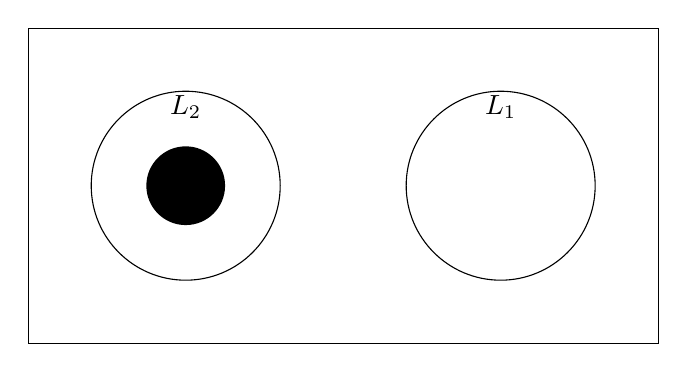
\begin{tikzpicture}
    % Outer rectangle
    \draw (0,0) rectangle (8,4);
    
    % Left egg shape with filled circle
    \draw (2,2) circle [x radius=1.2cm, y radius=1.2cm];
    \fill (2,2) circle [radius=0.5cm];
    
    % Right egg shape
    \draw (6,2) circle [x radius=1.2cm, y radius=1.2cm];   
    
    % Labels
    \node at (2,3) {$L_2$};
    \node at (6,3) {$L_1$};

\end{tikzpicture}

Consider the above image, the loop \( L_1 \) encloses a region outside the loop \(L_2 \) and the black part inside the loop \( L_2 \) denotes a region that has been cut off from the rectangle. Clearly the \(L_1\) loop can be shrunk to a point but the other one can't be shrunk to a point. Also these two loops cannot cross each other. 

The above is the study of Homotopy in Topology. Homotopy allows us to understand when two shapes or spaces can be continuously deformed into each other without tearing or gluing. It is a way of transforming one continuous function into another in a continuous manner. 

\begin{theorem}
    Two continuous functions \( f, g: X \rightarrow Y \) between topological spaces \( X \) and \( Y \) are said to be homotopic if there exists a continuous map \( H: X \times [0,1] \rightarrow Y \) such that:
\[ H(x, 0) = f(x) \]
\[ H(x, 1) = g(x) \]
for all \( x \in X \). The map \( H \) is called a homotopy between \( f \) and \( g \).
\end{theorem}

\subsection{Paths in Topology}

Let's move away from this for a moment and rethink our definition of path. 
\begin{theorem}
    A path from \( x_0 \in S \) to \( x_1 \in S \) in a topological space (S,U) is a continuous map \( \alpha(t): [0,1] \to S \) where \([0, 1]\) is the closed unit interval in the real numbers \(\mathbb{R}\). Such that 
    \[ \alpha(0) = x_0 \]
    \[ \alpha(1) = x_1\]
\end{theorem}

To be fair path is not an image but a function. We have the arbitrary freedom to chose our function but that has to map between topological space. 

\begin{theorem}
    A topological space \( S \) is said to be path-connected if for any two points \( x_0, x_1 \in S \), there exists a path \(\alpha\) such that \(\alpha(0) = x_0\) and \(\alpha(1) = x_1\). In other words, any two points in the space can be connected by a continuous path.
\end{theorem}

Now if a space is path connected then it is connected. Converse is not true. A space can be connected but not path connected. 

\subsection{Loops in Topology}
Now we move onto loops. Loops in topology is a closed path. Basically the starting and ending points/ sets are the same elements. 

\begin{theorem}
A \textit{closed path} or \textit{loop} in \(\mathcal{S}\) at \(x_0\) is a path \(\alpha(t)\) for which \(x_0 = x_1\), that is, \(\alpha(0) = \alpha(1) = x_0\). The loop is said to be \textit{based} at \(x_0\).
\end{theorem}

\begin{figure}
\centering
\begin{tikzpicture}

% Left circle
\draw (0,0) circle (1.5cm);
\node at (0,-1.7) {$t=0$};
\fill (0,-1.5) circle (0.05cm);
\node at (0,2) {$t=1/2$};
\node at (2.2,0) {$t=1/4$};
\node at (-2.2,0) {$t=3/4$};

% Arrow
\draw[->, thick] (2.3,0.2) to[out=30,in=150] node[above] {$\alpha(t)$} (4,0);

% Right shape
\begin{scope}[xshift=6cm]
\draw (0,0) to[out=90,in=180] (1,1) to[out=0,in=90] (2,0) to[out=270,in=0] (1,-1) to[out=180,in=270] cycle;
\fill (0,0) circle (0.05cm);
\node[anchor=north east] at (0,0) {$\alpha(0)=x_0$};
\draw (-2,-2) rectangle (2.5,1.5);
\end{scope}

\end{tikzpicture}
\caption{A based loop in a topological space $S$.}
\label{fig:based-loop}
\end{figure}

The idea of based at \( x_0 \) is very important. To multiply two loops we must have the condition that they are based at the same point. Otherwise they cannot be multiplied. We should also be careful in dealing the the \( \alpha(t) \). from the above definition. This is basically a space or collection of all possible functions or mappings. So we can have multiplie loops for the same based. 

\subsection{Loop Multiplication}
In topology, particularly in the study of the fundamental group, the multiplication of loops involves concatenating two loops to form a new loop, which in turn provides a group structure to the set of loops based at a given point. The formal definition is 

\begin{theorem}
Given a topological space \( X \) and a base point \( x_0 \in X \), let \(\alpha\) and \(\beta\) be two loops based at \( x_0 \). This means both \(\alpha\) and \(\beta\) are continuous maps \(\alpha, \beta: [0, 1] \to X\) such that \(\alpha(0) = \alpha(1) = x_0\) and \(\beta(0) = \beta(1) = x_0\).

The multiplication (or concatenation) of these loops, denoted \(\alpha * \beta\), is a new loop based at \( x_0 \) defined as follows:

\[
(\alpha * \beta)(t) = 
\begin{cases} 
\alpha(2t) & \text{for } 0 \leq t \leq \frac{1}{2}, \\
\beta(2t - 1) & \text{for } \frac{1}{2} < t \leq 1.
\end{cases}
\]
\end{theorem}

Why is it written like that. Its for abstraction and a more general handle on functions. 
For \( t \) in the first half of the interval \([0, 1]\), the loop \(\alpha * \beta\) follows the path of \(\alpha\) twice as fast (since \( \alpha(2t) \) covers the entire loop \(\alpha\) as \( t \) goes from \( 0 \) to \( \frac{1}{2} \)).
- For \( t \) in the second half of the interval \([0, 1]\), the loop \(\alpha * \beta\) follows the path of \(\beta\) twice as fast (since \( \beta(2t - 1) \) covers the entire loop \(\beta\) as \( t \) goes from \( \frac{1}{2} \) to \( 1 \)). So each of the \( \alpha, \beta \) individually obey the previous definitions. 

The inverse is also non-intuitive. Assuming the t value the \( \alpha(t) \) moves whatever it is in time t. Whereas, \( \alpha^{-1}(t) \) takes it back in time. So 

\[ \alpha^{-1}(t) = \alpha(1-t) \]

\subsection{Homotopy of Paths}

\begin{theorem}
    In topology, two paths \(\gamma_0\) and \(\gamma_1\) in a topological space \(X\), both starting at a point \(x_0\) and ending at a point \(x_1\), are said to be homotopic if one can be continuously deformed into the other. Formally, paths \(\gamma_0, \gamma_1: [0, 1] \to X\) are homotopic if there exists a continuous map \(H: [0, 1] \times [0, 1] \to X\) such that:

\[
H(t, 0) = \gamma_0(t), \quad H(t, 1) = \gamma_1(t) \quad \text{for all} \ t \in [0, 1],
\]

and

\[
H(0, s) = x_0, \quad H(1, s) = x_1 \quad \text{for all} \ s \in [0, 1].
\]

The map \(H\) is called a homotopy between \(\gamma_0\) and \(\gamma_1\).

\end{theorem}

Imagine stretching and bending a path \(\gamma_0\) to transform it into another path \(\gamma_1\), without breaking or lifting it from the space \(X\). This continuous deformation process is what a homotopy captures.

\begin{enumerate}
    \item \textbf{Reflexivity}: Every path is homotopic to itself.
    \item \textbf{Symmetry}: If \(\gamma_0\) is homotopic to \(\gamma_1\), then \(\gamma_1\) is homotopic to \(\gamma_0\).
    \item \textbf{Transitivity}: If \(\gamma_0\) is homotopic to \(\gamma_1\) and \(\gamma_1\) is homotopic to \(\gamma_2\), then \(\gamma_0\) is homotopic to \(\gamma_2\).
\end{enumerate}

\subsection{Homotopy of loops}

\begin{theorem}
A loop is a special kind of path that starts and ends at the same point, called the base point. Two loops \(\alpha_0\) and \(\alpha_1\) based at a point \(x_0\) in a topological space \(X\) are said to be homotopic if there exists a continuous map \(H: [0, 1] \times [0, 1] \to X\) such that:

\[
H(t, 0) = \alpha_0(t), \quad H(t, 1) = \alpha_1(t) \quad \text{for all} \ t \in [0, 1],
\]

and

\[
H(0, s) = H(1, s) = x_0 \quad \text{for all} \ s \in [0, 1].
\]

The map \(H\) is called a homotopy between \(\alpha_0\) and \(\alpha_1\).
\end{theorem}

For loops, the homotopy provides a way to continuously deform one loop into another while keeping the base point fixed. Imagine taking a rubber band looped around a fixed peg at \(x_0\) and transforming its shape continuously without lifting it off the peg.

Consider the unit circle \(S^1\). Any loop based at a point on the circle can be thought of as a map \(\alpha: [0, 1] \to S^1\) with \(\alpha(0) = \alpha(1)\). The loop that winds around the circle once counterclockwise is homotopic to the loop that winds around it once clockwise, but they belong to different homotopy classes if the winding numbers (how many times they wrap around the circle) are considered.

A clearer example would be two fixed points on a circle. We can pass a circle and if done properly we can fit a parabola or ellipse as well. All of these are then termed homotopic. 
They start and end at the same base point. 

Mathematically, if two loops \( \alpha \& \beta \) are homotopic to each other then, 

\[ \alpha \dot \sim \beta \]

homotopy is an equivalence relation. 

\begin{theorem}

\begin{enumerate}
    \item \textbf{Reflexivity}:
    \begin{itemize}
        \item Any loop is homotopic to itself. Mathematically, \(\alpha \dot \sim \alpha\).
    \end{itemize}

    \item \textbf{Symmetry}:
    \begin{itemize}
        \item If loop \(\alpha\) is homotopic to loop \(\beta\), then loop \(\beta\) is homotopic to loop \(\alpha\). Mathematically, if \(\alpha \dot \sim \beta\), then \(\beta \dot \sim \alpha\).
    \end{itemize}

    \item \textbf{Transitivity}:
    \begin{itemize}
        \item If loop \(\alpha\) is homotopic to loop \(\beta\) and loop \(\beta\) is homotopic to loop \(\gamma\), then loop \(\alpha\) is homotopic to loop \(\gamma\). Mathematically, if \(\alpha \dot \sim \beta\) and \(\beta \dot \sim \gamma\), then \(\alpha \sim \gamma\).
    \end{itemize}

    \item \textbf{Continuous Deformation}:
    \begin{itemize}
        \item Two loops \(\alpha\) and \(\beta\) are homotopic if there exists a continuous function \(H: S^1 \times [0, 1] \to X\) such that:
        \begin{itemize}
            \item \(H(s, 0) = \alpha(s)\) for all \(s \in S^1\),
            \item \(H(s, 1) = \beta(s)\) for all \(s \in S^1\),
            \item \(H(s, t)\) is continuous in both \(s\) and \(t\).
        \end{itemize}
    \end{itemize}

    \item \textbf{Base Point Preservation}:
    \begin{itemize}
        \item In the context of loops in a pointed space \((X, x_0)\), homotopy between loops must preserve the base point. This means that the base point \(x_0\) must remain fixed throughout the deformation:
        \begin{itemize}
            \item \(H(x_0, t) = x_0\) for all \(t \in [0, 1]\).
        \end{itemize}
    \end{itemize}

\end{enumerate}
    
\end{theorem}

To define a class of loops which are all homotopic to some loop \( \alpha \) is given by the notation \( [\alpha] \)


\subsection{Fundamental Group}

The \textbf{fundamental group} of a topological space \( S \) with a chosen base point \( x_0 \) is a mathematical structure that reflects the different ways in which one can traverse loops in the space starting and ending at \( x_0 \). It is denoted as \( \pi_1(S, x_0) \).


Formally, the fundamental group \( \pi_1(S, x_0) \) is the set of all equivalence classes of loops based at \( x_0 \), where two loops are considered equivalent if one can be continuously deformed into the other (i.e., they are homotopic):

\[
\pi_1(S, x_0) = \left\{ [\alpha] \mid \alpha(t) \text{ is a loop in } S \text{ based at } x_0 \right\}
\]

This is a group cause it has the following properties. 
\begin{enumerate}
    \item \textbf{Closure}: \[  [\alpha] \in \pi_1, \quad [\beta] \in \pi_1 \implies [\alpha] \star [\beta] = [\alpha \star \beta] \in \pi_1 \]

    \item \textbf{Identity}:  \([i]\) is the equivalence class of loops homotopic to the constant loop at \(x_0\). Clearly
        \[
        [\alpha] \star [i] = [i] \star [\alpha] = [\alpha \star i] = [\alpha]
        \]
        for all \([\alpha]\).

    \item \textbf{Inverse}:  \[
    [\alpha]^{-1} = [\alpha^{-1}], \text{ because }   \]
    \[  [\alpha]^{-1} \star [\alpha] = [\alpha^{-1} \star \alpha] = [i] \]

    \item \textbf{Associativity}: \[ ([\alpha] \star [\beta]) \star [\gamma] = [\alpha] \star ([\beta] \star [\gamma]) \]
\end{enumerate}

Also \(  [\alpha] \star [\beta] \neq [\beta] \star [\alpha] \) meaning this is not an Abelian Group. 

\subsubsection*{Examples}

\begin{itemize}
    \item \textbf{Simply Connected Spaces}: A space is simply connected if every loop can be contracted to a point. For such spaces, the fundamental group is trivial, consisting only of the identity element. An example is \(\mathbb{R}^n\) for \(n \geq 1\).

    \item \textbf{Circle \(S^1\)}: The fundamental group of the circle \(S^1\) is isomorphic to the integers \(\mathbb{Z}\). Each integer \(n\) corresponds to the loop that winds around the circle \(n\) times.
\end{itemize}

To proceed further, we will find it useful to define the product operation even on paths which are \textit{not} closed, namely, paths \(\alpha(t)\) such that \(\alpha(0)\) and \(\alpha(1)\) are distinct. 

\begin{theorem}
The \textit{product} of two open paths \(\alpha(t)\) and \(\beta(t)\) is defined only if \(\alpha(1) = \beta(0)\), in other words, if the final point of \(\alpha\) is the same as the initial point of \(\beta\), and is given by \(\gamma = \alpha \star \beta\) where:
\[
\gamma(t) = 
\begin{cases} 
\alpha(2t), & 0 \leq t \leq \frac{1}{2} \\
\beta(2t - 1), & \frac{1}{2} \leq t \leq 1
\end{cases} \quad 
\]

\end{theorem}

Here, the initial point of the product path \(\alpha \star \beta\) is the initial point of \(\alpha\), and the final point of \(\alpha \star \beta\) is the final point of \(\beta\).

Now we look to the fundamental groups once again. In principle this group depends on the base point with respect to which it is defined. Thus, \(\pi_1(S, x_0)\) is a different group from \(\pi_1(S, x_1)\) for \(x_0 \neq x_1\). But in fact under very general conditions the two are the same. 

To specify what we mean by two groups being the "same", let us first define the concept of "homomorphism" between groups (not to be confused with "homeomorphism" between topological spaces!). This is a mapping from one group to another which preserves the group operations. 

\begin{theorem}
    
If \(G\) and \(H\) are two groups, a \textit{homomorphism} \(\phi: G \to H\) is a map \(g \in G \rightarrow \phi(g) \in H\) such that:
\[
\begin{aligned}
&\phi: g^{-1} \in G \implies \phi(g^{-1}) = (\phi(g))^{-1} \in H \\
&\phi: g_1 \cdot g_2 \in G \implies \phi(g_1 \cdot g_2) = \phi(g_1) \cdot \phi(g_2) \in H \\
&\phi: i \in G \implies \phi(i) = i' \in H
\end{aligned}
\]
    
\end{theorem}

Homomorphism preserves group multiplication. We cannot say from homomorphism that G and H are the same group. They can or cannot be the same group. But there is a stronger condition called Isomorphism. 

\begin{theorem}
    A homomorphism \(\phi\) is an \textit{isomorphism} if it is also bijective (one-to-one and onto). If an isomorphism exists between two groups, the groups are said to be \textit{isomorphic}, and can be thought of as completely equivalent to each other.    
\end{theorem}

If there exists an isomorphism between G \& H, then effectively G \& H are the same group. So in other words they can be transformed onto one other. 

Now we can show the following 

\begin{theorem}
    If a topological space \( S \) is \textit{path-connected} then \(\pi_1(S, x_0)\) and \(\pi_1(S, x_1)\) are isomorphic as groups.

\textbf{Proof:} 
Consider \(\alpha(t)\) based at \(x_0\) along with its equivalence class \([\alpha] \in \pi_1(S, x_0)\). Let \(\gamma(t)\) be an open path from \(x_0\) to \(x_1\). Now define a map
\[
\phi : \pi_1(S, x_0) \to \pi_1(S, x_1) \quad \]
by
\[
\phi([\alpha]) = [\gamma^{-1} \star \alpha \star \gamma] \quad \]
Clearly \([\alpha] \in \pi_1(S, x_0) \implies \phi([\alpha]) \in \pi_1(S, x_1)\). And moreover this is an isomorphism. For example, the product law holds:
\[
\begin{aligned}
\phi([\alpha] \star [\beta]) &= \phi([\alpha \star \beta]) \\
&= [\gamma^{-1} \star \alpha \star \beta \star \gamma] \\
&= [\gamma^{-1} \star \alpha \star \gamma \star \gamma^{-1} \star \beta \star \gamma] \\
&= \phi([\alpha]) \star \phi([\beta]) \quad 
\end{aligned}
\]
with \([\alpha], [\beta] \in \pi_1(S, x_0)\). 

\end{theorem}

Similarly one can check the other properties of a homomorphism, as well as the fact that this map is bijective which finally makes it an isomorphism.

Because of the above theorem, for path-connected spaces we denote the fundamental group as \(\pi_1(S)\) instead of \(\pi_1(S, x_0)\). It must be kept in mind, however, that in the process of finding \(\pi_1\) we must always work with loops based at some (arbitrary) point \(x_0\). The final result for \(\pi_1\) will then be independent of \(x_0\).

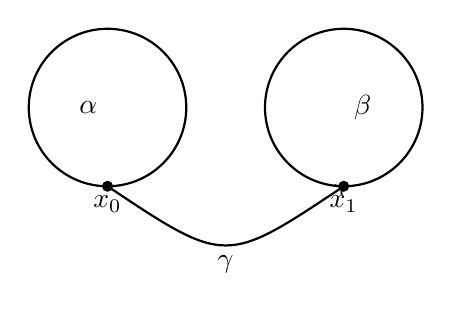
\begin{tikzpicture}
    % Draw the loops
    \draw[thick] (0,0) circle(1) node[left] {$\alpha$};
    \draw[thick] (3,0) circle(1) node[right] {$\beta$};
    
    % Draw the points
    \fill (0,-1) circle(2pt) node[below] {$x_0$};
    \fill (3,-1) circle(2pt) node[below] {$x_1$};
    
    % Draw the path gamma
    \draw[thick,->] (0,-1) .. controls (1.5,-2) .. (3,-1) node[midway, below] {$\gamma$};
\end{tikzpicture}

To understand what just happened we consider the terminologies once more. A path-connected space is a type of space where any two points can be joined by a continuous path. Whereas fundamental group \(\pi_1\) represents different "shapes" of loops that can be drawn from a starting point (base point) in the space and then return to the starting point without crossing edges or boundaries. These loops are looked at up to deformation, meaning one loop can be "stretched" or "squeezed" but not broken, into another.

The above theorem states that if you have a path-connected space \(S\), the fundamental group at any two points \(x_0\) and \(x_1\) in \(S\) are essentially the same, or in mathematical terms, "isomorphic." This isomorphism means there's a way to convert loops based at \(x_0\) to loops based at \(x_1\) without losing any fundamental properties of those loops. The way loops are transformed between two points involves "dragging" them along a path \(\gamma\) from \(x_0\) to \(x_1\).

In the diagram two loops \(\alpha\) and \(\beta\) based at points \(x_0\) and \(x_1\) respectively are connected by a path \(\gamma\). The transformation (or map) \(\phi\) defined in the proof essentially takes a loop at \(x_0\), drags it to \(x_1\) using \(\gamma\), then drags it back to \(x_0\), ensuring that the loop's nature remains unchanged. This dragging involves tracing the path to \(x_1\) (using \(\gamma\)), following the loop, and then coming back via the reverse path (\(\gamma^{-1}\)).

\subsection{Homotopy Types} 
The homotopy concept extends naturally to pairs of maps between any two topological spaces.

\begin{theorem}

 Let \(S\) and \(T\) be two topological spaces. For two continuous functions
\[
f_0: S \rightarrow T \quad \text{and} \quad f_1: S \rightarrow T,
\]
we say \(f_0\) and \(f_1\) are \textit{homotopic} if there exists a continuous map
\[
F: S \times [0, 1] \rightarrow T,
\]
such that the following conditions hold:
\[
F(x, 0) = f_0(x) \quad \text{and} \quad F(x, 1) = f_1(x).
\]
\end{theorem}

In the particular case where \(S\) is the closed interval \([0, 1]\), homotopy of functions simplifies to homotopy of paths or loops, but it's important to note that these do not rely on a fixed base point. Hence, we use the symbol \(\sim\) to denote the homotopy of functions described here, which should not be confused with based homotopy of loops denoted by the same symbol in other contexts.

Exploring homotopy between maps in various topological spaces helps us uncover properties shared between those spaces, which may not be immediately apparent.

Now we can define the homotopy of two topological spaces 

\begin{theorem}
Two topological spaces \( S \) and \( T \) belong to the same \textit{homotopy type} if there are continuous functions 
\[
f: S \rightarrow T \quad \text{and} \quad g: T \rightarrow S
\]
such that the compositions \( f \circ g \) and \( g \circ f \) are homotopic to the identity maps on \( T \) and \( S \) respectively. We denote these conditions as:
\[
f \circ g: T \to T \sim \text{i}_T \quad \text{and} \quad g \circ f: S \to S \sim \text{i}_S,
\]
where \( \text{i}_T \) and \( \text{i}_S \) are the identity maps on \( T \) and \( S \).

\end{theorem}

This characteristic of having the same homotopy type ensures that the fundamental groups of \( S \) and \( T \), denoted \( \pi_1(S) \) and \( \pi_1(T) \), are isomorphic. 

\begin{theorem}
If \( S \) and \( T \) are path-connected spaces with the same homotopy type, then their fundamental groups are isomorphic:
\[
\pi_1(S) \cong \pi_1(T).
\]    
\end{theorem}

This isomorphism indicates a deep connection between the spaces in terms of their loop structures and overall topology, despite potential differences in their geometries.

\begin{theorem}
If \( S \) and \( T \) are homeomorphic as topological spaces, then they share the same homotopy type, and consequently, their fundamental groups \( \pi_1 \) are identical. This follows because homeomorphism involves a pair of continuous maps \( f: S \to T \) and \( g: T \to S \) such that \( g = f^{-1} \), satisfying:
\[
f \circ g = \text{i}_T, \quad g \circ f = \text{i}_S.
\]
This establishes that \( S \) and \( T \) are homotopy equivalent.    
\end{theorem}
Now why do we need topology. Answer becomes apparant from the above discussion. Homotopy is topological invariant. Two spaces which are topologically equivalent (homeomorphic) have the same homotopy properties. However, the converse is not necessarily true. Two topological spaces may have the same \( \pi_1 \), but this does not imply that they are homeomorphic. 

We will need a few more definitions. Those are given below. 

\begin{theorem}
\textbf{1. } A Topological space is \textit{contractible} if it is homotopy equivalent to a single point.  

\textbf{2. } A topological space \( S \) is called \textit{simply connected} if its fundamental group \( \pi_1(S) \) is trivial, i.e., \( \pi_1(S) = \{i\} \), where \( i \) is the identity element. If \( \pi_1(S) \) contains more than the identity element, the space is \textit{multiply connected}.

\end{theorem}

Simply connected spaces are characterized by the absence of nontrivial loops: all loops can be continuously deformed into a point within the space. For a contractible space \( S \), the fundamental group \( \pi_1(S) \) is trivial, i.e., \( \pi_1(S) = \{i\} \). Therefore, such a space is simply connected. However, the converse is not always true; a simply connected space need not be contractible. We will explore this through examples below.

some examples to check homotopy and contractible spaces. 

\textbf{Example 1:} $\mathbb{R}^n$ is a Contractible Space

To show that $\mathbb{R}^n$ is a contractible space, we need to demonstrate that there exists a homotopy between the identity map on $\mathbb{R}^n$ and a constant map. A topological space is defined as contractible if it is homotopy equivalent to a point.

Here's how we can construct such a homotopy for $\mathbb{R}^n$:

Let $f: \mathbb{R}^n \to \mathbb{R}^n$ be the identity map, $f(x) = x$, and let $g: \mathbb{R}^n \to \mathbb{R}^n$ be a constant map, $g(x) = x_0$ for some fixed $x_0 \in \mathbb{R}^n$.

We need to find a continuous function $H: \mathbb{R}^n \times [0, 1] \to \mathbb{R}^n$ such that:
\begin{enumerate}
    \item $H(x, 0) = f(x) = x$ for all $x \in \mathbb{R}^n$,
    \item $H(x, 1) = g(x) = x_0$ for all $x \in \mathbb{R}^n$.
\end{enumerate}


Define $H$ by:
\[ H(x, t) = (1 - t)x + tx_0 \]
where $x \in \mathbb{R}^n$ and $t \in [0, 1]$.

\begin{itemize}
    \item \textbf{Continuity}: The map $H$ is clearly continuous as it is a linear combination of continuous functions $x$ and $x_0$, and scalar multiplication and addition in $\mathbb{R}^n$ are continuous operations.
    \item \textbf{Boundary Conditions}:
    \begin{itemize}
        \item At $t = 0$, $H(x, 0) = (1 - 0)x + 0 \cdot x_0 = x$, which is the identity map.
        \item At $t = 1$, $H(x, 1) = (1 - 1)x + 1 \cdot x_0 = x_0$, which is the constant map.
\end{itemize}
\end{itemize}

Since such a homotopy $H$ exists, we can conclude that $\mathbb{R}^n$ is homotopy equivalent to a single point, which implies that $\mathbb{R}^n$ is a contractible space. This demonstrates that all loops in $\mathbb{R}^n$ can be continuously shrunk to a point, and thus $\mathbb{R}^n$ has trivial homotopy groups, confirming its contractibility.

\textbf{Example 2:} 2-Sphere $S^2$ is not contractible 

To discuss the contractibility of a topological space, one must demonstrate the possibility to continuously deform every point in the space into a single point, effectively reducing the entire space to a point.

\[
S^2 = \{(x,y,z) \in \mathbb{R}^3 \mid x^2 + y^2 + z^2 = 1\}.
\]

A potential strategy to contract $S^2$ could involve moving every point to the south pole along great circles. However, this approach encounters a critical issue at the north pole, which cannot be moved in any direction without disrupting the continuity of the map. This obstacle implies that $S^2$ cannot be contracted to a point.

Despite this, any loop on $S^2$, based at any point, can be continuously shrunk to a point. This property indicates that the fundamental group of $S^2$ is trivial:

\[
\pi_1(S^2) = \{i\}.
\]

Thus, while $S^2$ is simply connected, implying that there are no non-trivial loops, its inability to be contracted to a single point due to the obstruction at the poles demonstrates that $S^2$ is \textbf{not contractible}.

\textbf{Example 3:} Circle $S^1$ is not contractible 

Consider \( S^1 \) as the set of all points in \( \mathbb{R}^2 \) at a unit distance from the origin. \( S^1 \) is not contractible and possesses a non-trivial fundamental group.

Define a loop \( \alpha_n: [0,1] \rightarrow S^1 \) where \( \alpha_n \) wraps around the circle \( n \) times. For \( n > 0 \), the loop winds \( n \) times anticlockwise; for \( n < 0 \), it winds \( |n| \) times clockwise; and for \( n = 0 \), \( \alpha_0 \) is the constant loop at a point \( x_0 \in S^1 \).

The fundamental group \( \pi_1(S^1) \) can be visualized by considering the homotopy classes of these loops. Two loops \( \alpha_n \) and \( \alpha_m \) are distinct in homotopy if \( m \neq n \), reflecting different numbers of wrappings around the circle, which cannot be homotopically deformed into one another.

The group operation in \( \pi_1(S^1) \) corresponds to the concatenation of loops, leading to the relation:
\[
[\alpha_n] * [\alpha_m] = [\alpha_{n+m}],
\]
where the right-hand side represents a loop that winds \( n+m \) times around the circle. This operation exhibits the structure of the integers \( \mathbb{Z} \) under addition. Formally, we have an isomorphism:
\[
\pi_1(S^1) \cong \mathbb{Z}.
\]
This isomorphism maps the homotopy class \( [\alpha_n] \) to the integer \( n \), known as the winding number of the loop.

Since \( \pi_1(S^1) \) is isomorphic to \( \mathbb{Z} \) and not trivial, \( S^1 \) is not contractible. A contractible space would have a trivial fundamental group, which is clearly not the case here. The presence of multiple, non-homotopic loops arising from different numbers of wrappings around the circle illustrates the rich topological structure of \( S^1 \) and confirms its non-contractible nature.

The above basically states take a coin and try to wrap the circular side using a rubber band twice or thrice. Then the question is can the rubber band deform to a single point or to a single loop structure. Obviously no, It cannot be morphed into a single loop without cutting a part of the rubber band. That's the argument used to prove that the loops on $S^1$ are not homotopic thus not contractible. 

\section{Differentiable Manifolds-I}

\subsection{Idea of Manifolds}

A topological space is a set equipped with a structure that allows us to talk about continuity and connectedness. The simplest examples are lines (\(\mathbb{R}\)) and planes (\(\mathbb{R}^2\)). If two spaces are homeomorphic, they must share key topological properties, like dimension. Dimension is a topological property. Consider, \(\mathbb{R}\) and \(\mathbb{R}^2\). By deleting a point from both, \(\mathbb{R} \setminus \{0\}\) becomes two disjoint intervals (disconnected), while \(\mathbb{R}^2 \setminus \{0\}\) remains connected. This difference in behavior upon the removal of a point helps prove that they are not homeomorphic, meaning they do not have the same topological dimension. \(S^1\) and \(\mathbb{R}\) are not homeomorphic, nor are \(S^2\) and \(\mathbb{R}^2\), again through arguments involving connectivity after removing points. Though \(S^1\) and \(S^2\) are not globally homeomorphic to \(\mathbb{R}\) and \(\mathbb{R}^2\) respectively, they are locally homeomorphic. This means in small enough neighborhoods, these behave like Euclidean spaces of their respective dimensions. 

\begin{theorem}
Let \( M \) be a topological space. A \textit{chart} \( C \) on \( M \) is a collection \( (U, \phi, n) \) such that:
\begin{enumerate}
    \item[(i)] \( U \) is an open set of \( M \).
    \item[(ii)] \( \phi \) is a homeomorphism: \( U \subseteq M \rightarrow \phi(U) \subseteq \mathbb{R}^n \). (Thus, \( \phi(U) \) is open in \( \mathbb{R}^n \).)
    \item[(iii)] \( n \) is a positive integer, called the \textit{dimension} of the chart \( C \).
\end{enumerate} 

\end{theorem}
In plain language, a chart is a piece of the topological space, with a homeomorphism equating it to a piece of some Euclidean space. 

It is evident that \( \mathbb{R}^n \) comes with a preferred choice of coordinates, called \textit{Cartesian coordinates}, namely the \( n \) real numbers specifying each point. Now given a chart, each point on it can be labelled by considering the image of this point in \( \mathbb{R}^n \) and then using the Cartesian coordinates of that point.

\begin{theorem}
    
Given a chart \( C = (U, \phi, n) \), the \textit{coordinates} of a point \( p \in U \subseteq M \) are the Cartesian coordinates in \( \mathbb{R}^n \) of the point \( \phi(p) \) in \( \phi(U) \subseteq \mathbb{R}^n \). When we allow the points \( p \) to vary over \( U \), the Cartesian components of \( \phi(p) \) in \( \mathbb{R}^n \) define a set of \( n \) real-valued functions on \( U \subseteq M \) called \textit{coordinate functions}.
    
\end{theorem}

The concept of chart has enabled us to locally map a piece of a topological space to \( \mathbb{R}^n \). A function on this piece of the topological space can then be differentiated by simply differentiating, in the familiar sense, the components of the coordinate functions defined above.

In simpler terms, this definition is about how we can understand and analyze shapes that might be more complex than standard shapes like planes or spheres. The idea of a "chart" is a tool in mathematics that helps us map a piece of a complicated shape onto a simpler, flat space like \(\mathbb{R}^n\) (which could be a line, plane, or higher-dimensional space). 

Think of a chart as a way of flattening a small part of a curved surface so that it looks like a regular flat piece of paper. This allows us to use simple calculus, which we usually do on flat surfaces, even on curved surfaces. When we use a chart, each point on our original shape gets a set of coordinates, just like on a flat grid. These coordinates are what we call "coordinate functions." Since one chart can only cover a part of the whole shape, we use many such charts to cover the entire shape. This way, we can apply calculus everywhere on the shape, not just where one chart is. By using multiple charts to cover an entire shape, we ensure that we can perform calculus operations (like differentiation) across the whole surface, no matter how complex its geometry might be. 

\begin{theorem}
Let \( C_1 = (U_1, \phi_1, n) \) and \( C_2 = (U_2, \phi_2, n) \) be two charts on \( M \). Then \( C_1 \) and \( C_2 \) are ``\(C^\infty\)-compatible'' or simply ``compatible'' if:
\begin{enumerate}
    \item[(i)] \( U_1 \cap U_2 = \emptyset \), or
    \item[(ii)] the maps \( \phi_1 \circ \phi_2^{-1} : \phi_2(U_1 \cap U_2) \rightarrow \phi_1(U_1 \cap U_2) \) and \( \phi_2 \circ \phi_1^{-1} : \phi_1(U_1 \cap U_2) \rightarrow \phi_2(U_1 \cap U_2) \) are infinitely differentiable (\( C^\infty \)) functions.
\end{enumerate}    
\end{theorem}

\begin{figure}
    \begin{center}
        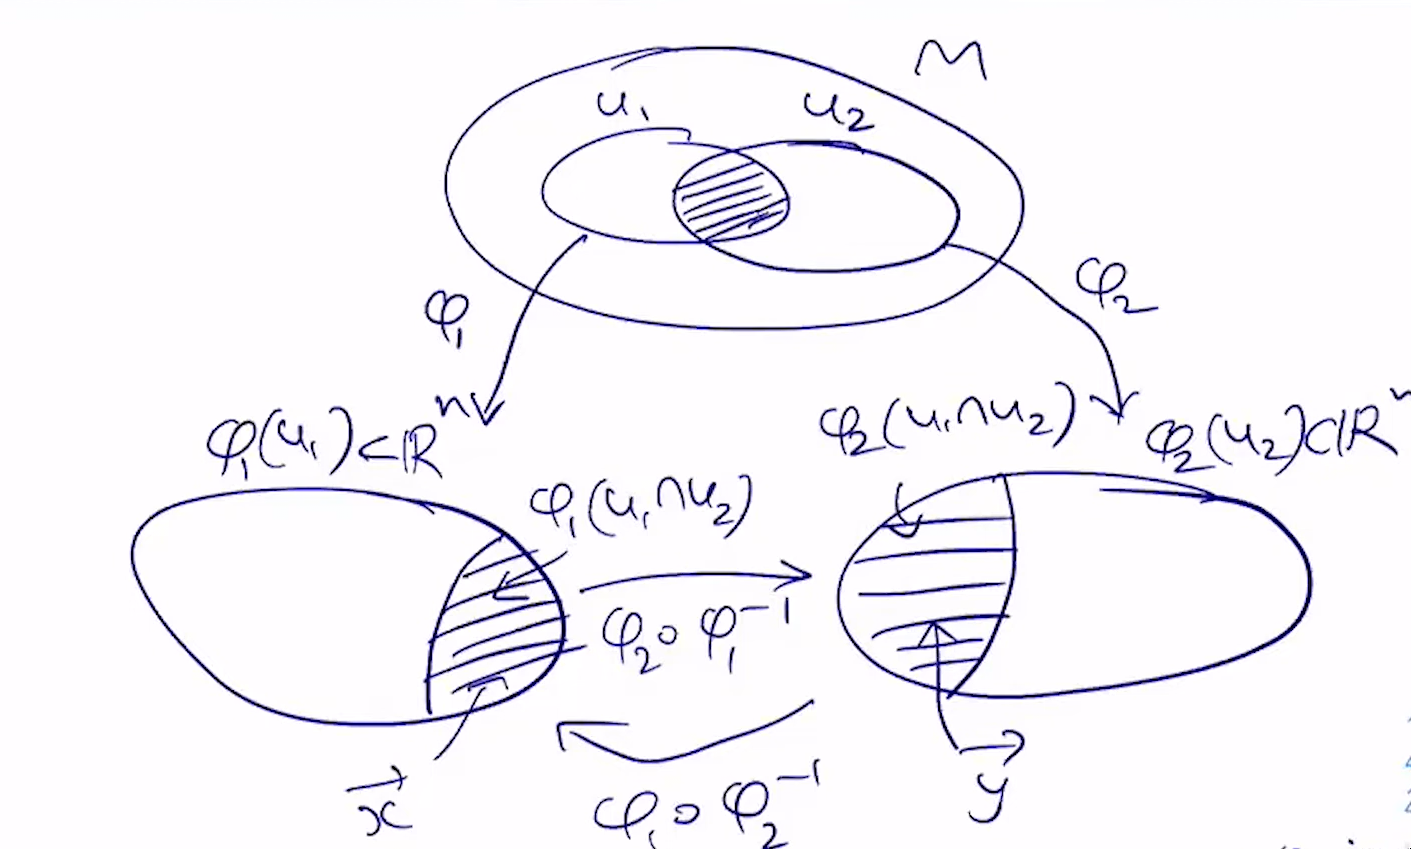
\includegraphics[width=0.95\textwidth]{figures/def_manifold.png}
    \end{center}
    \caption{Definition of a Manifold}\label{fig:definition_manifold}
\end{figure}

In the figure, consider that some person used the shaded region of the M space and converted/transformed or cut or whatever terminology is relevent, and gets the left part of the shaded region in $\phi_1(u_1)$ this is basically the same as saying that the person just wrote the physical law in terms of variable $\vec{x}$. Now another person can do the same thing maybe in a different coordinate system or different frame and will get the right portion $\vec{y}$. Since they are overlappong and are the same thing we now have a relation between two coordinates $\vec{x} \& \vec{y}$. They can now be transformed or differentiated. 

\begin{theorem}
    A \(C^\infty\)-atlas \( \mathcal{U} \) on a topological space \( M \) is a family of charts \( (U_\alpha, \phi_\alpha, n) \) which covers \( M \), so that \( \bigcup_\alpha U_\alpha = M \), such that all the charts in the family are mutually \(C^\infty\)-compatible.

    Two \(C^\infty\)-atlases are said to be \textit{compatible} (with each other) if every chart of one atlas is compatible with every chart of the other atlas.

\end{theorem}
A \(C^\infty\)-atlas on a topological space \(M\) is a collection of charts that together cover the entire space \(M\). Each chart in this collection maps a part of \(M\) into Euclidean space \(\mathbb{R}^n\). The superscript \(C^\infty\) indicates that the charts are smooth, meaning that the transition maps between any two overlapping charts are infinitely differentiable.

The map \(\phi_\alpha\) essentially provides a coordinate system for each part of the manifold. The union of all open sets \(U_\alpha\) in the atlas equals the entire manifold, ensuring no part of \(M\) is left out. The charts must smoothly align where they overlap. If you transition from one chart to another where they overlap, this transition must be smooth (infinitely differentiable).

Two \(C^\infty\)-atlases are considered compatible if every chart in one atlas is compatible with every chart in the other atlas. This means that for any pair of overlapping charts, one from each atlas, the transition map between them must be infinitely differentiable.

Compatibility is essential for defining a consistent structure on the manifold that doesn't depend on the choice of atlas. If two atlases are compatible, they essentially provide the same "smooth structure" to the manifold, allowing for a unified approach to calculus and analysis on \(M\).

An interesting property of atlases and charts are that for \(C^\infty\)-compatibility is an equivalence relation. It implies three key things:

1. \textbf{Reflexivity}: Every atlas is \(C^\infty\)-compatible with itself. The transition maps within a single atlas are, by definition of the atlas being a \(C^\infty\)-atlas, infinitely differentiable.

2. \textbf{Symmetry}: If atlas A is \(C^\infty\)-compatible with atlas B, then atlas B is \(C^\infty\)-compatible with atlas A. This means that if you can transition smoothly from charts in A to charts in B, the reverse transitions are also smooth.

3. \textbf{Transitivity}: If atlas A is \(C^\infty\)-compatible with atlas B, and atlas B with atlas C, then atlas A is \(C^\infty\)-compatible with atlas C. This ensures that smooth structures can be extended across multiple atlases, maintaining a consistent differentiable structure throughout.

But for charts, the key issue arises in the physical extent of the overlap and the specific transition functions used. Suppose \(A\) overlaps with \(B\) in one region and \(B\) overlaps with \(C\) in a different region. There may be no direct overlap between \(A\) and \(C\), or the overlap between \(A\) and \(C\) might involve different sections of these charts that were not "tested" via the transitions through \(B\). This can lead to situations where direct transitions between \(A\) and \(C\) are not smooth, even though transitions through \(B\) are smooth. 

\begin{theorem}
    A differentiable structure of class \(C^\infty\) on a topological space \(M\) is an equivalence class of \(C^\infty\)-compatible atlases on \(M\).     
\end{theorem}

It is always easier to study equivalence classes if we can find a unique representative of each class in some way, since this can then be used to label the class. We may pick a unique atlas out of each equivalence class of compatible atlases as follows: take the union of all atlases in a class and call it the \textit{maximal atlas}. Then a differentiable structure is just a choice of maximal atlas \(U\) on \(M\). This choice therefore labels the differentiable structure.

We are finally in a position to define a manifold.

\begin{theorem}
    A differentiable manifold is a Hausdorff topological space and an equivalence class of atlases.    
\end{theorem}

Now, what is going on? Lets start with the terminologies. 

A topological space is termed "Hausdorff" if any two distinct points in the space can be separated by disjoint open sets. This separation means that no two points can be arbitrarily close without being the same. A manifold is equipped with an atlas, which is a collection of charts that together cover the entire manifold. Each chart provides a way to coordinate or "chart" part of the manifold, typically mapping it to an open subset of Euclidean space (\(\mathbb{R}^n\)). An equivalence class of atlases refers to a group of atlases where any atlas in the group can be smoothly transformed into any other through their transition maps. This means all atlases in this class provide a consistent way to study the manifold’s structure, enabling calculus and other analyses.
It doesn't matter which atlas from the class you choose to use; they all describe the manifold in a way that is consistent with each other in terms of smoothness and differentiability.

Combining these two characteristics, the definition describes a space that not only has a straightforward and well-defined topological nature (Hausdorff) but also allows for smooth calculus operations anywhere on the manifold due to its differentiable structure (given by the equivalence class of \(C^\infty\) atlases).

\begin{theorem}
\textbf{Properties of Differential Manifolds}:
\begin{enumerate}
    \item It is locally Euclidean.
    \item It is locally compact (every point \( x \in M \) has a compact neighbourhood).
    \item An open subset \( U \subseteq M \) is itself a differentiable manifold, called an ``open submanifold''.
    \item The product of two manifolds is well-defined (using Cartesian products).
\end{enumerate}
\end{theorem}

\textbf{\(\mathbb{R}^n\) is a Differentiable Manifold}

1. \textbf{Locally Euclidean:} By definition, any point in \(\mathbb{R}^n\) has a neighborhood that looks exactly like \(\mathbb{R}^n\), fulfilling the locally Euclidean condition directly.

2. \textbf{Atlas and Charts:} For \(\mathbb{R}^n\), we can use a single chart covering the entire space where the chart map \(\phi\) is the identity map \(\phi: \mathbb{R}^n \rightarrow \mathbb{R}^n\)

3. \textbf{Smooth Compatibility:} Since we only have one chart, and it maps to itself by the identity function, the compatibility condition (smooth transitions between charts) is automatically satisfied.

4. \textbf{Hausdorff and Second-countable:} The space \(\mathbb{R}^n\) is Hausdorff as any two distinct points can be separated by disjoint open sets. It is second-countable as it has a countable basis (e.g., open balls with rational radii centered at points with rational coordinates).

Hence, \(\mathbb{R}^n\) is a differentiable manifold.

\textbf{Proving \(S^1\) is a Differentiable Manifold}

1.\textbf{Locally Euclidean:}  Each point on \(S^1\) (defined as \(S^1 = \{(x, y) \in \mathbb{R}^2 : x^2 + y^2 = 1\}\)) has a neighborhood that resembles an open interval in \(\mathbb{R}\), satisfying the locally Euclidean condition.

2. \textbf{Atlas and Charts:} We can cover \(S^1\) with two charts to avoid the coordinate singularity at one point (commonly taken at \( (1,0) \) and \((-1,0)\)):
   - Chart \(U_1 = S^1 \setminus \{(1,0)\}\) with coordinates given by the projection onto the y-axis, or an angular coordinate excluding the angle corresponding to \((1,0)\).
   - Chart \(U_2 = S^1 \setminus \{(-1,0)\}\) similarly defined.

3. \textbf{Smooth Compatibility:} The transition maps between these two charts (moving from one angular coordinate to another excluding different points) are smooth, involving simple arithmetic operations on the angles.

4.\textbf{Hausdorff and Second-countable:}  \(S^1\), as a subspace of \(\mathbb{R}^2\), inherits the Hausdorff property. It is also second-countable as it can be covered by a countable union of open arcs.

Thus, \(S^1\) is a differentiable manifold.

\subsection{Differentiation of functions} 

\begin{figure}
    \begin{center}
        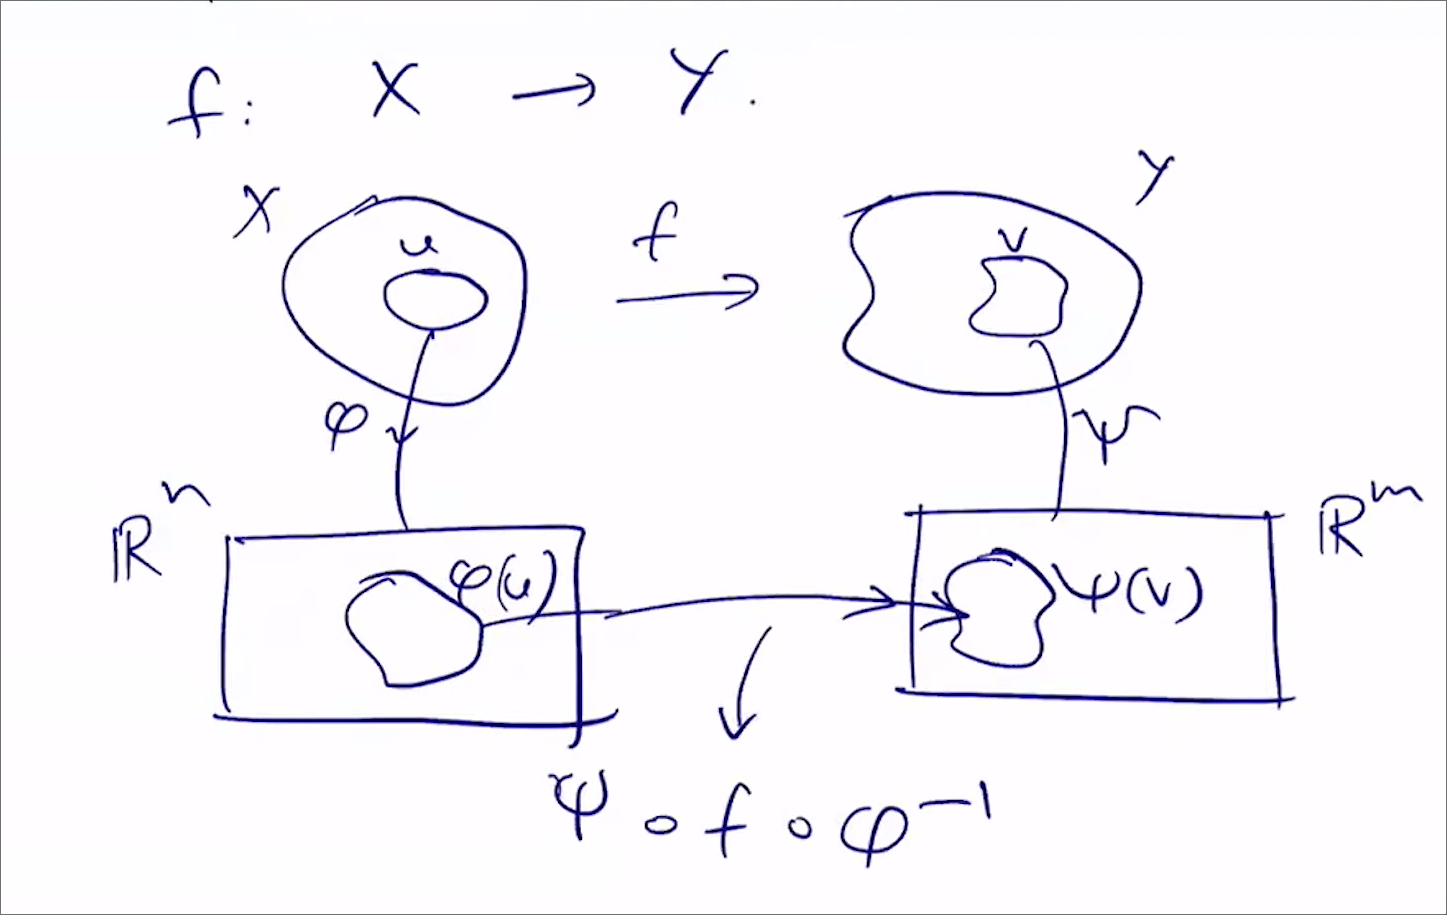
\includegraphics[width=0.95\textwidth]{figures/eq_manifolds.png}
    \end{center}
    \caption{}\label{fig:}
\end{figure}

In the context of manifolds, we define a function to be differentiable in a manner analogous to functions in Euclidean space. However, since manifolds may not have global coordinate systems, we rely on local coordinates provided by charts.

\begin{theorem}
A function \( f: X \to Y \) between manifolds is said to be differentiable if the function \(\psi \circ f \circ \phi^{-1} : \mathbb{R}^n \to \mathbb{R}^m\) is differentiable in the usual sense. Here, \(\phi\) and \(\psi\) are chart maps for manifolds \(X\) and \(Y\), respectively, translating manifold coordinates into Euclidean coordinates where standard calculus applies.
\end{theorem}

Diffeomorphisms are a special type of mapping between manifolds that not only preserve the structure of the manifolds but also allow for the smooth translation of geometric and analytic properties between them.

\begin{theorem}
    Two manifolds \(X\) and \(Y\) are said to be diffeomorphic if there exists a function \(f: X \to Y\) such that:
    \begin{enumerate}
        \item[(i)] \(f\) is a homeomorphism, ensuring a one-to-one, onto, and continuous mapping with a continuous inverse.
        \item[(ii)] Both \(f\) and \(f^{-1}\) are \(C^\infty\), meaning they are smooth; this includes having all derivatives exist and be continuous.
    \end{enumerate}
\end{theorem}

\subsection{Orientability}
Orientability of a manifold refers to the possibility of consistently defining what it means to be clockwise or counterclockwise across the entire manifold.

\begin{figure}
    \begin{center}
        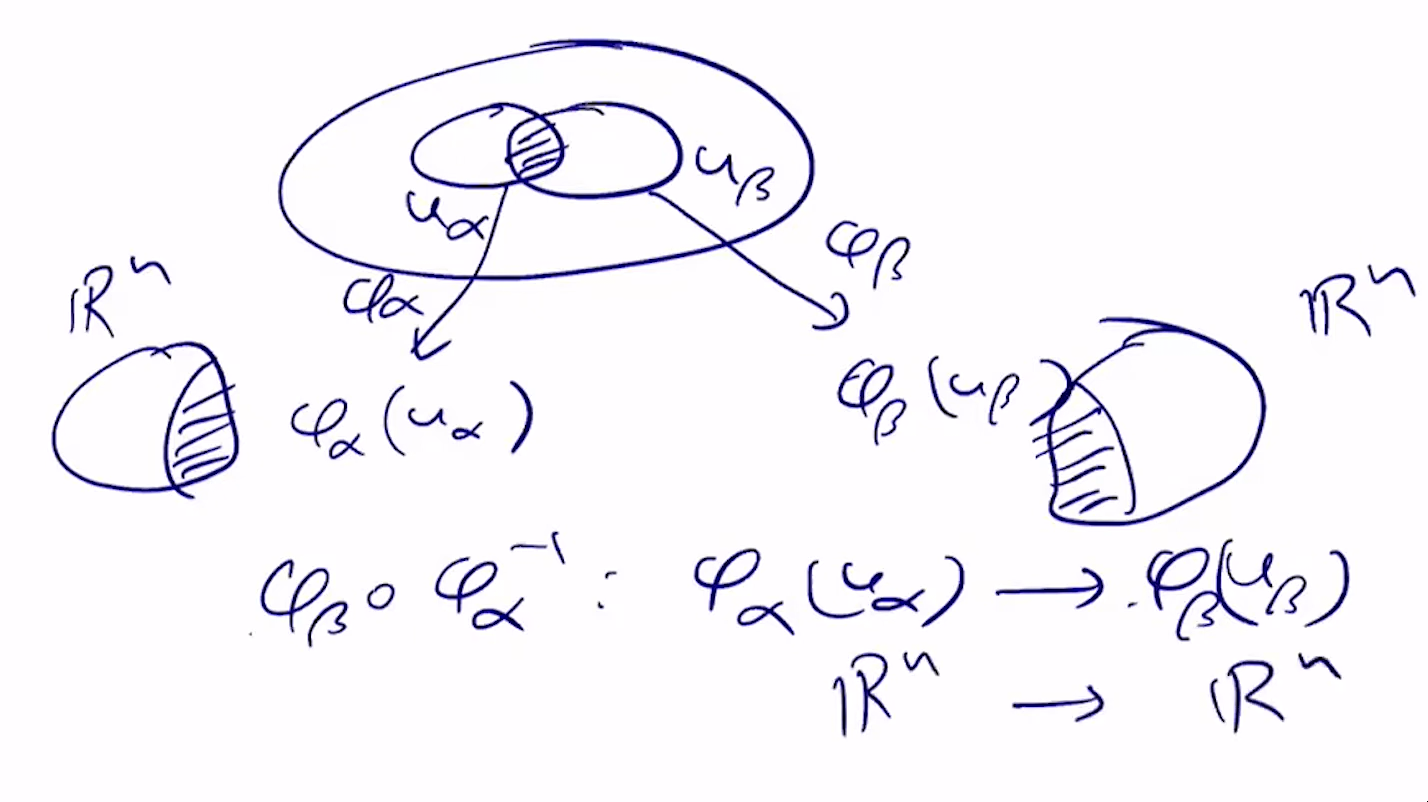
\includegraphics[width=0.95\textwidth]{figures/orientation.png}
    \end{center}
    \caption{}
\end{figure}

\begin{theorem}
    A manifold is \textit{orientable} if an atlas can be chosen such that for every overlap of charts, the transition map \(\phi_{\beta} \circ \phi_{\alpha}^{-1} : \mathbb{R}^n \rightarrow \mathbb{R}^n\) has a positive Jacobian determinant. This positive determinant indicates that orientation is preserved between overlapping charts.
\end{theorem}

\subsection{Calculus on manifolds}

While local regions of manifolds look like Euclidean space, the global topology can significantly differ. Ordinary calculus doesn't directly address how to define derivatives when the underlying space (manifold) can curve or loop back on itself.
How to handle calculations across manifold charts, where local Euclidean views must seamlessly connect through transition maps. Nor does it help in computing derivatives that respect the manifold's intrinsic geometry, which can be critical in physics for understanding phenomena like gravity or electromagnetism in curved spacetime. To address these issues, calculus on manifolds formalizes and extends the concepts of differentiation and integration to work in curved spaces. 

\subsubsection{Tangent Vectors and Tangent Space} 

The concept of a differentiable manifold is crucial because it allows us to apply calculus as we do in $\mathbb{R}^n$, thanks to local equivalence. To manage this, we employ coordinate charts to transition from manifold calculus to $\mathbb{R}^n$. The main complexity arises in transferring calculations between multiple charts that cover the manifold.

Consider a real-valued function $f : M \rightarrow \mathbb{R}$ on a manifold $M$. Within a coordinate patch, this function corresponds to a map $\mathbb{R}^n \rightarrow \mathbb{R}$. Changing the coordinate system alters the function representation:
\[
f' : y^i \in \mathbb{R}^n \rightarrow f'(y^i) \in \mathbb{R},
\]
where the transformation on overlapping charts for a different coordinate is defined by:
\[
f'(y^i) = f(x^i).
\]
Differentiating $f$ in a coordinate patch $\varphi_\alpha(U_\alpha)$ gives:
\[
\frac{\partial f}{\partial x^i} : \varphi_\alpha(U_\alpha) \rightarrow \mathbb{R}.
\]
Though $f$ is coordinate invariant, its derivatives transform differently:
\[
f'(y) = f(x) \Rightarrow \frac{\partial f'}{\partial y^i} = \frac{\partial f}{\partial x^i} \frac{\partial x^i}{\partial y^i} \neq \frac{\partial f}{\partial x^i}.
\]

To better grasp this, consider a parametrized curve $p(t) \subseteq M$, which in a coordinate patch maps to $x^i(t) \subseteq \mathbb{R}^n$. The tangent vector at $t_0$ is defined as $dx^i/dt |_{t=t_0}$, encapsulating the rate and direction of motion at that point. 

\begin{theorem}
In a coordinate patch, the tangent vector to a curve $p(t) \subseteq M$ is $dx^i/dt$, derived from the coordinates $x^i(t)$ of the curve's image $\varphi_\alpha(p(t))$.
\end{theorem}

Tangent vectors transform between overlapping patches as follows:
\[
\frac{dx^i}{dt} \rightarrow \frac{dy^i}{dt} = \frac{\partial y^i}{\partial x^j} \frac{dx^j}{dt},
\]
making the tangent vector's meaning invariant across different coordinates, a property known as "covariance". We simply mean the tangent is now in a coordinate-less representation. 

\textbf{Vector Space of Tangent Vectors:} Tangent vectors at a single point form a vector space. We can have a \( n>=1 \) number of tangents drawn in any direction. Combining tangent vectors from two intersecting curves $p(t)$ and $q(t)$ at $t_0$ generates a new vector:
\[
a^i(x_0) = \left[ \frac{dx^i}{dt} (p(t)) + \frac{dx^i}{dt} (q(t)) \right]_{t=t_0},
\]
This describes a straight line in $\mathbb{R}^n$:
\[
x^i(t) = x_0^i + a^i(x_0)t.
\]
Here \( x_0 \) is the image of the point \( p(0) \) on the manifold. This line can be mapped back to $M$, forming a new curve around the intersection point of $p(t)$ and $q(t)$, using $\varphi_\alpha^{-1}$.

\begin{theorem}
The set of all tangent vectors at a point $p \in M$ constitutes the tangent space $T_p(M)$.

Tangent vectors are constructed by:
\begin{enumerate}
    \item Choosing a point $x_0^i \in \mathbb{R}^n$ and defining a curve such that $\left. \frac{dx^i}{dt} \right|_{t=t_0} = a^i$.
    \item Lifting this curve to $M$ using $\varphi_\alpha^{-1}$.
    \item In another coordinate system, redefining the vector components to maintain consistency across transformations.
\end{enumerate}    
\end{theorem}

Combining the differentiation of functions with tangent vector analysis on $M$ provides a coordinate invariant definition of a tangent vector. The derivative of a function $f$ along a curve is a coordinate-independent differential:
\[
\frac{df}{dt} = \frac{df}{dx^i} \frac{dx^i}{dt} (p(t)),
\]

Thus, the derivative of $f$ along a curve, at some point, is expressed in terms of its gradient $\frac{\partial f}{\partial x^i}$ in the chosen coordinate system, contracted with the tangent vector at that point. But while both $\frac{\partial f}{\partial x^i}$ and $\frac{dx^i}{dt}$ are coordinate-dependent objects, when contracted together they give $\frac{df}{dt}$ which is manifestly coordinate independent. 

Now, 
\[
\frac{df}{dt} = \left[ \frac{dx^i}{dt} (p(t)) \right] \left[ \frac{\partial}{\partial x^i} \right] f.
\]
This operator, $\frac{dx^i}{dt} (p(t)) \frac{\partial}{\partial x^i}$, maps any $C^\infty$ functions on a manifold to a new functions on the curve and is termed a vector field when generalized over the manifold. The linearity and distribution over function multiplication define and characterize vector fields:
\[
X(fg) = (Xf)g + f(Xg).
\]


\end{document}

